%%
%% Author: jemanj
%% 3/29/19
%%

% Preamble
\documentclass[11pt]{article}

% Packages
\usepackage{amsmath}
\usepackage{graphicx}
\usepackage{caption}
\usepackage[]{bm}
\usepackage{float}
\usepackage[margin=1in]{geometry}

\title{Learning to time (LeT): A tutorial}
\author{Emmanuel Alcalá}
% Document
\begin{document}

    \maketitle

    \section{States dynamics}

LeT have three components:

    \begin{itemize}
        \item A series of (behavioral) states.
        \item Associative links connecting states to a operant response.
        \item The operant response
    \end{itemize}

The states advance at a rate $\lambda$, which is a normal random variable.

    \[
        \lambda \sim \mathcal{N} (\mu, \sigma),\; \lambda > 0
    \]

    The symbol $\sim$ means "distributed as", and $\mathcal{N}$ is for the Normal Density Function, but often referred
    as \textit{normal distribution}, not to be confused with the \textit{cumulative distribution function}.
    Every $i$-th trial, a value $\lambda_i$ is sampled and the trial advance from $t = 1$ until $T$, the time of reinforcement, so that the
reinforced state is $N(t = T)$.
    The states transitions form the random process $N(t) = \lceil {\lambda t} \rceil$.
    The $N$ states starts at 1 and are activated serially.

There are no upper bound of the states that can be activated, so the limits of $N(t)$ are determined by $\mu$ and $\sigma$.
For example, if $\mu = 1$ \footnote{Which means the rate $\lambda$ most probable value is 1 state per second.} and $\sigma = 0.1$, the states will be very close to the true $T$, but if $\sigma = 0.6$,
there will be more reinforced states that are far from $T$, and $N(t)$ spans over a broader set of values.
Figure 1 shows a simulation with $\mu=1,\sigma=0.2$.
    Note that if $\mu > 1$ the mean of the reinforced states (dotted line in the histogram of Figure 1) will be shifted above $T$, or below if $\mu < 1$.

Thus, the reinforced states $N(t = T)_i$ (or $N(T)_i$ for short) of the $i$-th trials, is the vector
$\mathbf{N^*} = \boldsymbol{\lambda} T$.

    \begin{figure}[H]
            \centering
            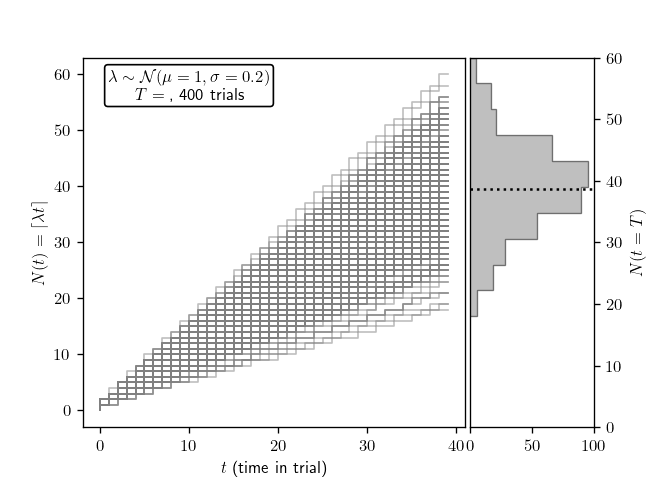
\includegraphics[scale=0.7]{nt_let}
            \caption{Example of a process of 400 trials. The left panel shows the state transitions for every
                    $\lambda$ sampled from the normal distribution (see the textbox inset). At $t = 40$, the reinforced
                    states spread around the true value of $T$ (40 s), so they approximate a normal distribution with mean
                    $\mu \times t$ and standard deviation $\sigma \times t$ (right panel).}
    \end{figure}
    The states below $N(t)$ are extinguished, and the states above are inactive.
    There is a $q(n,T)$ probability that the state $n$ is extinguished at $T$, and a probability $p(n,T)$ that it is reinforced.
    Also, there is a $r(n,T)$ probability that the $n$ state will be inactive (i.e., the trial will end before $T$, and
    state $n$ will not be reinforced nor extinguished).
    All need sum to 1, so that $p(n,T) = 1 - q(n,T) - r(n,T)$.

Because $n$ is extinguished if and only if (\textit{iif}) $n < N(T)$, so $q(n,T) = p(n < N(T))$,
and $N(T) = \lceil \lambda T \rceil$, we have

    \[
        q(n,T) = P \Big(\lambda > \frac{n}{T}\Big) = 1 - P(\lambda < \frac{n}{T}) = 1 - \Phi \Big (\frac{n}{T}, \mu, \sigma \Big)
    \]


On which $\Phi (\cdot)$ is the \textit{cumulative distribution function (CDF)}, or just \textit{distribution function}:

    \[
        \Phi \Big( \frac{n}{T}, \mu, \sigma \Big) = \frac{1}{\sigma \sqrt{2 \pi}} \int\limits_{-\infty}^{\frac{n}{T}} \exp^{-(x - \mu)/2\sigma^2}dx
    \]

But since $t > 0$, we are just interested in evaluate the integral in the domain (0,$\frac{n}{T}$] \footnote{Of course,
    we should subtract first the integral of the domain $[-\infty, 0]$, but is a very small quantity, so it's negligible.}.
$\Phi$ doesn't have a closed form solution, and it's often approximated by Taylor expansion with

    \[
        \exp^{u} = \sum^{k=0}_{\infty} \frac{u^k}{k!}, \; \text{for } u = \frac{-(x - \mu)}{2 \sigma^2}
    \]

But we are modern people and will take advantage of the software.
Most statistical packages can compute CDFs.
Let's see an example.
If $\mu = 1, \sigma = 0.2, n = 15$
and $T = 40$, $q(15,40) = P \Big( \lambda > \frac{15}{40} \Big)$ or $1 - \Phi(\frac{15}{40},1,0.2)$. Using \textsf{Python}:

    \begin{verbatim}
        from scipy.stats import norm
        1 - norm.cdf(n/T,loc=1,scale=0.2)
    \end{verbatim}

Returns 0.99911, that is, the probability (actually, the density, or the area under the curve, etc) of state 15 being a
    extinguished state is very high.
    We can also interpret that quantity in terms of expected proportion of trials with state
    15 not reinforced.
    See Figure 2 for a graphical representation of this probability just calculated.

    \begin{figure}[H]
        \centering
        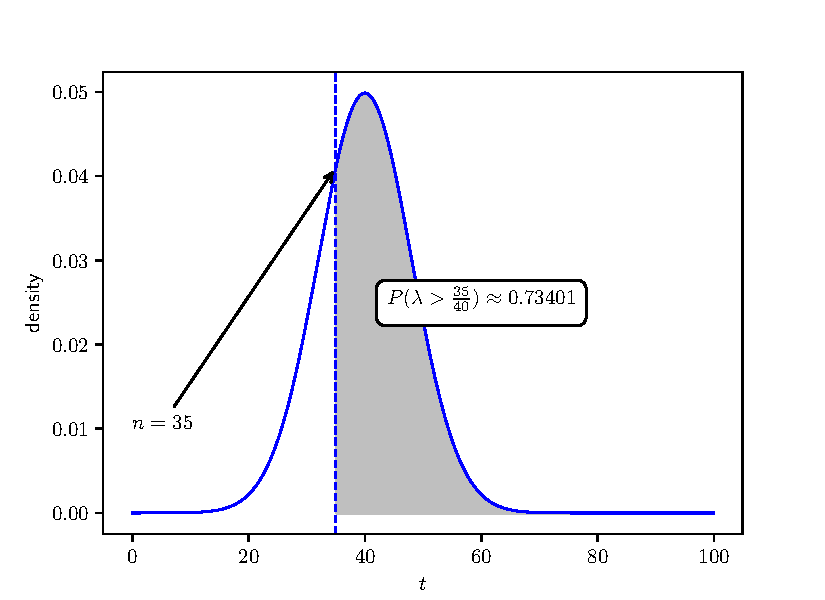
\includegraphics[scale=0.65]{lambda_nT}
        \caption{Probability density function of a normal distribution with $\mu = 1, \sigma = 0.2$ for $t = 1,2,3..,40$.
        Shaded area shows the density $P(\lambda > 15/40)$, which means that is \textit{highly} probable that state 15
        is a extinguished state.}
    \end{figure}

    The state $n$ is inactive \textit{iif} $n > N(T)$, and, again, $N(T) = \lceil \lambda T \rceil$.
    Because $\lceil \lambda T \rceil$ is a quantity greater than $\lambda T$, we can express $n > \lceil \lambda T \rceil$
    as $n - 1 > \lambda T$ to avoid that rounding $\lceil \lambda T \rceil$ give us $n$.
    Then, the probability that $n$ is inactive, or $r(n,T)$, is

    \[
        r(n,T) = P(n > \lceil \lambda T \rceil) = P(n - 1 > \lambda T) = \Phi \Big( \frac{n-1}{T},\mu,\sigma \Big)
    \]

    Now, the expresion for the probability that $n$ will be reinforced can be expressed as

    \[
        p(n,T) = \Phi \Big ( \frac{n}{T}, \mu, \sigma \Big) - \Phi \Big ( \frac{n - 1}{T},\mu,\sigma \Big)
    \]

    In Machado, Malheiro and Erlhagen (2009) the authors provide an approximation of $p(n,T)$ without saying how they
    achieved that solution. The approximation is

    \[
        p(n,T) \approx \frac{1}{T} \mathcal{N} \Big(\frac{n}{T},\mu,\sigma \Big)
    \]
\end{document}